\documentclass[main.tex]{subfiles}
\begin{document}
\section{Adaptive Signal Processing}


\subsection{The Least Mean Square (LMS) Algorithm}

When studying non-linear signals, adaptive filters that approximate the Wiener solutions are considered. The primary focus here will be on the Least Mean Squared (LMS) algorithm, which recursively adjusts the weights following the gradient method of optimisation. Essentially, the weights are updated according to the following equation;

\begin{align*}
w(n+1) &= w(n) - \mu \frac{\partial}{\partial w}\left( \frac{1}{2}e^2(n) \right),\ \ \ \ \ \ n=0,1,...  \\
&= w(n) + \mu e(n) x(n) \numberthis \label{equation-lms}
\end{align*}

where $e(n) = x(n) - \hat{x}(n)$. In what followed, we look at the LMS algorithm under a number of circumstances and try to ensure that conversion is always possible and reasonably fast. % TODO: quanitfy this



\subsubsection{Correlation Matrix for AR(2) Process}

To find the auto-correlation matrix $\textbf{R}$ of the input vector $\textbf{x}(n)=[x(n-1),\ x(n-2)]^T$ for a AR(2) proccess, the following defitions are first made. From $\textbf{R} = E\left[\textbf{x}(n)\textbf{x}^T(n)\right]$,

\begin{align*}
\textbf{R} = E \left\{ \left[
\begin{array}{cc}
x[n-1]^2 & x[n-1]x[n-2]  \\
x[n-2]x[n-1] & x[n-2]^2  \end{array}
\right]
\right\}
&=
\left[
\begin{array}{cc}
E \left\{ x[n-1]^2 \right\} & E \left\{x[n-1]x[n-2] \right\} \\
E \left\{ x[n-2]x[n-1]\right\} & E \left\{x[n-2]^2 \right\} \end{array}
\right]\\
&= 
\left[
\begin{array}{cc}
\gamma(0) & \gamma(1) \\
\gamma(1) & \gamma(0) \end{array}
\right]
\end{align*}

From here, we can consider %TODO: \cite{Garc2012a};

\begin{align}
x(n) = a_1*x(n-1) + a_2*x(n-2) + \eta(n)
\label{corr-mtx-base}
\end{align}	

Two tricks are now used to find $\gamma(0)$ and $\gamma(1)$. To find the variance, $\gamma(0)$, both sides of equation~\ref{corr-mtx-base} are squared and the expectation is taken. To find $\gamma(1)$, each side is multiplied by a $x(n-1)$ term \footnote{ A more general trick that is useful for finding the auto-correlation function for any distance can be done by multiplying eq~\ref{corr-mtx-base} by $x(n-k)$TODOcite{Cochrane1997a}. This gives the result $\gamma(k) = a_1\gamma(k-1) + a_2\gamma(k-2)$. However, it is more intutive and helpful to look at the two individual cases of $\gamma = 0,1$. }.

\begin{align*}
E\left[x^2(n)\right] &= \gamma(0) = E\left[  (a_1x(n-1) + a_2x(n-2) + \eta(n))^2  \right]\\
&= E\left[a_1^2x^2(n-1) + a_2^2x^2(n-2) + 2a_1a_2x(n-1)x(n-2) + 2a_1x(n-1)\eta(n) + 2a_2x(n-2)\eta(n) + \eta^2(n)\right]\\
&= a_1^2\gamma(0) + a_2^2\gamma(0) + 2a_1a_2\gamma(1) + \sigma^2\\
\\
E\left[x(n)x(n-1)\right] &= \gamma(1) = E\left[  a_1x(n-1)x(n-1) + a_2x(n-2)x(n-1) + \eta(n)x(n-1)  \right]\\
&= a_1\gamma(0) + a_2\gamma(1)
\end{align*}


Substituting $a_1 = 0.1, a_2 = 0.8, \sigma_n^2 = 0.25$, the following equations are solved,
\begin{align*}
\gamma(0) = 0.1^2\gamma(0) + 0.8^2\gamma(0) + 2(0.1)(0.8)\gamma(1) + 0.25\\
\gamma(1) = 0.1\gamma(0) + 0.8\gamma(1)
\end{align*}
 
Which results in $\gamma(0) = 25/27$ and $\gamma(1) = 25/54$, such that

\begin{equation}
\textbf{R} = \left[
\begin{array}{cc}
\gamma(0) & \gamma(1) \\[6pt]
\gamma(1) &  \gamma(0) \end{array}
\right] = \left[
\begin{array}{cc}
\frac{25}{27} & \frac{25}{54} \\[6pt]
\frac{25}{54} &  \frac{25}{27} \end{array}
\right]
\end{equation}

\paragraph{To find the convergence in the mean,} a maximum value for $\mu$ is estimated with $2/(trace(\textbf{R}))$, such that $0 \leq \mu \leq \frac{2}{trace(\textbf{R})}$. This gives $0 \leq \mu \leq \frac{729}{625} = 1.1664$.

A more precise method to do this is to look at the eigenvalues of the auto-correlation matrix. This is however computationally expensive, and generally not favourable (especially for high-order systems). In our case, these are $\mathbf{ \lambda } = [0.4630, 1.3889] ^ T $, which leads to $0 \leq \mu \leq \frac{2}{\lambda_{max}} = 1.43999$ with the maximum convergence speed\footnote{Speed here generally does not make it a good choice - a high $\mu$ leads to instability and large fluctuations.}.  at $\mu = \frac{2}{\lambda_{max} + \lambda_{min}} = 1.08$






\subsubsection{Implementation of LMS Adaptive Predictor}

Over 1000 samples, the performance of the LMS-algorithm for parameter prediction can be calculate by looking at the squared prediction errror. To do this, a $\mu$ value of $0.01$ and $0.05$ is considered. Both a single run of the algorithm, as well as an averaged error over 100 iterations of the algorithm, are shown.


\begin{figure}[H]
	\centering
	\begin{subfigure}[b]{0.45\textwidth}
		\resizebox{\textwidth}{!}{\input{matlabimages/3_1_b_1_iterations.tikz}}
	\end{subfigure}%
	~ %add desired spacing between images, e. g. ~, \quad, \qquad, \hfill etc.
	%(or a blank line to force the subfigure onto a new line)
	\begin{subfigure}[b]{0.45\textwidth}
		\resizebox{\textwidth}{!}{\input{matlabimages/3_1_b_100_iterations.tikz}}
	\end{subfigure}
	\caption{Squared Prediction Error of the LMS over 1 and 100 iterations.}
	\label{fig:1-1-b}
\end{figure}



As expected, the higher value of $\mu$ converges faster (as it's learning parameters change more rapidly)\footnote{Faster changes are not always good - a higher value of $\mu$ sometimes leads to instability}. It's interesting to note that for both values of $\mu$, the error reaches values near $-6dB$. This is from the fact that our noise is from $var(\sigma_n^2 = 0.25)$, and $10*log_{10}(0.25) = -6.021$.


\subsubsection{Misadjustment Rate}


As seen in figure~\ref{fig:1-1-b}, it can be seen that the error term tends to fluctuate around the minimum sqare error ($\sigma_n^2$). However, there is an excess to this error, which is dubbed the excess mean square error (EMSE), defined as $EMSE = MSE - \sigma_2^2$. The \textbf{misadjustment rate} is simply the ratio between the EMSE and the minimum mean square error.

\begin{equation}
\mathcal{M} = \frac{EMSE}{\sigma_n^2}
\end{equation}

Looking over the estimated and the caluclated values for the misadjustment rate, it can be seen that they lie within the same order of magnitude. Furthermore, as the value of $\mu$ increases, as does the misadjustment rate. This comes from the fact that steady state fluctuations are more likely due to a larger step.

\begin{table}[h]
	\centering
	\begin{tabular}{ | c |  c | }
		\hline
		$\mathcal{M}$ \textit{(calculated)} & $\hat{\mathcal{M}}_{LMS}$ \textit{(estimate)} \\ \hline
		0.008395      & 0.00926                   \\ \hline
		0.043028      & 0.04630                  \\ \hline
	\end{tabular}
\end{table}










\subsubsection{Steady State Filter Coefficients}

Over 100 independant trials of the LMS algorithm, the mean values of the estimated filter coefficients $\hat{a}_1$ and $\hat{a}_2$ are plotted. As shown, the coefficients approach the actual values with only $a_2$ estimated with 4\% error (estimated in both cases as 0.77, rather than 0.8).

\begin{figure}[H]
	\centering
	\begin{subfigure}[b]{0.45\textwidth}
		\resizebox{\textwidth}{!}{\input{matlabimages/3_1_d_mu0_01.tikz}}
		\caption{Filter Coefficients for $\mu = 0.01$}
	\end{subfigure}%
	~ %add desired spacing between images, e. g. ~, \quad, \qquad, \hfill etc.
	%(or a blank line to force the subfigure onto a new line)
	\begin{subfigure}[b]{0.45\textwidth}
		\resizebox{\textwidth}{!}{\input{matlabimages/3_1_d_mu0_05.tikz}}
		\caption{Filter Coefficients for $\mu = 0.05$}
	\end{subfigure}
	\caption{Approximation of the filter coefficients using the LMS algorithm. Results are averaged over 500 independant trials.}
	\label{fig:animals}
\end{figure}










\subsubsection{Leaky LMS}

The cost function used in the standard LMS algorithm does not always converge. TODO: When does it not. A work-around in these situations is to look at changing the error function to include a leakage term, allowing for convergance. 

In this situation, the error function that is to be minimised is change to include an additional term; $J_2(n) = \frac{1}{2}(e^2(n) + \gamma||w(n)||^2_2)$. From here, it is trivial to prove that the weights update according to $\textbf{w}(n+1) = (1-\mu \gamma)\textbf{w}(n) + \mu e(n)\textbf{x}(n)$.

Starting with;


\begin{align*}
\textbf{w}(n+1) &= \textbf{w}(n) - \mu\frac{\partial J_2}{\partial w}\\
\textbf{w}(n+1) &= \textbf{w}(n) - \mu\left(\frac{\partial}{\partial w}\left[\frac{1}{2}e^2(n)\right] + \frac{\partial}{\partial w}\left[\frac{1}{2}\gamma||\textbf{w}(n)||^2_2\right]\right)\\
\textbf{w}(n+1) &= \textbf{w}(n) - \mu\left(\left[-e(n)\textbf{x}(n)\right] + \left[\gamma\textbf{w}(n)\right]\right)\\
\textbf{w}(n+1) &= \textbf{w}(n) - \mu\gamma\textbf{w}(n) + \mu e(n)\textbf{x}(n)\\
\textbf{w}(n+1) &= (1-\mu\gamma)\textbf{w}(n) + \mu e(n)\textbf{x}(n)
\end{align*}







\subsubsection{Implementation}

\begin{figure}[H]
	\centering
	\begin{subfigure}[b]{0.45\textwidth}
		\resizebox{\textwidth}{!}{\input{matlabimages/3_1_f_mu0_01.tikz}}
		\caption{Filter Coefficients for $\mu = 0.01$}
	\end{subfigure}%
	~ %add desired spacing between images, e. g. ~, \quad, \qquad, \hfill etc.
	%(or a blank line to force the subfigure onto a new line)
	\begin{subfigure}[b]{0.45\textwidth}
		\resizebox{\textwidth}{!}{\input{matlabimages/3_1_f_mu0_05.tikz}}
		\caption{Filter Coefficients for $\mu = 0.05$}
	\end{subfigure}
	\caption{Approximation of the filter coefficients using the Leaky LMS algorithm. Results are averaged over 100 independant trials.}
	\label{fig:animals}
\end{figure}



Though the values do approach the original filter parameters $[0.1, 0.8]$, there is a considerably larger bias when compared to the original LMS filter. In the normal LMS filter, a maximum error of around 4\% was seen - however, in the leaky LMS, both coefficients show a bias of around 10\% to 30\%.

The large error factor is explained by the addition of the leak factor $-\mu\gamma\textbf{w}(n)$, which continually reduces the strength of the weights, even in steady state. In fact, it can be shown that the convergence of the weights is related to a corrupted version of the correlation matrixTODOcite{Kamenetsky2004}:

\begin{align*}
\lim_{k \to \inf}E(\textbf{w}(n)) = (\textbf{R} + \gamma \textbf{I})^{-1}\textbf{p}
\end{align*}

where $\textbf{I}$ is the identity matrix and $\textbf{p}$ the cross correlation vector. The additional corruption of the auto-correlation matrix allows it to be inverted, but yields biased results.

% TODO: define cross correlation


















\subsection{Adaptive Step Sizes}

In the above section, a constant step size $\mu$ was selected. It should be noted that a higher step size will converge to the correct answer sooner, but can overshoot and cause instability when set too high. A lower one will converge more slowly, but will tend to be more stable once converegence has been achieved. As such, a desirable trait in the step size is to allow them to be adaptive; i.e. higher before convergence, and lower after convergence. 

To this purpose, three algorithms are investiaged. Each algorithm adaptively updates the step, $\mu(n)$, according to the following equations:

\begin{align}
\textbf{w}(n+1) &= \textbf{w}(n) + \mu(n)e(n)\textbf{x}(n)\\
\text{with\ \ \ \ } \mu(n+1) &= \mu(n) + \rho e(n) \textbf{x}^T(n)\mathbf{\psi}(n)
\end{align}

with

\begin{align*}
\text{Benveniste:\ \ }      \mathbf{\psi}(n) &= [\textbf{I} - \mu(n-1)\textbf{x}(n-1)\textbf{x}^T(n-1)]\mathbf{\psi}(n-1)+e(n-1)x(n-1)\\
\text{Ang \& Farhang:\ \ }  \mathbf{\psi}(n) &= \alpha\mathbf{\psi}(n-1) + e(n-1)\textbf{x}(n-1)\\
\text{Matthews \& Xie:\ \ } \mathbf{\psi}(n) &= e(n-1)\textbf{x}(n-1)\\
\end{align*}



	
\subsubsection{Implementation of Adaptive Step Sizes}

\begin{figure}[H]
	\centering 
	\resizebox{\textwidth}{!}{\input{matlabimages/3-2-a.tikz}}
	\caption{Comparison of original LMS and adaprive step sized LMS using the Benveniste, Ang \& Farhang and Matthews \& Xie approaches.}
	\label{fig:q3_2_a}
\end{figure}

As expected, the adaptive step size algorithms outperform the standard LMS. From figure~\ref{fig:q3_2_a}, it can be seen that the adaptive step sizes converge with a similar speed as the LMS algorithm with $\mu = 0.1$. However, though they converge at the same speed, all three adaptive step sizes outperform the LMS at steady state, with the error being significantly lower. 



\subsubsection{Normalised LMS (NLMS)}

As the weight update for the LMS algorithm ($\Delta w$) is proportional to the magnitude of the input vector $\textbf{x}(n)$, it's not uncommon to normalise the step size. This is done by dividing $\Delta w$ by the magnitude of the input vector, summed with a regularisation factor $\epsilon$ to ensure stability of the algorithm even when the input is 0.

\begin{equation}
\textbf{w}(n+1) = \textbf{w}(n) + \frac{\beta}{\epsilon + ||\textbf{x}(n)||^2}e(n)\textbf{x}(n) \label{eq:3-2-2-nlms}
\end{equation}

By starting with an updated function that relied on the \textit{a posteriori} error, such that $\textbf{w}(n+1) = \textbf{w}(n) + \mu e_p(n)\textbf{x}(n)$, with $e_p(n) = d(n) - \textbf{x}^T(n)\textbf{w}(n+1)$, it can be shown that this is an implementation of the NLMS algorithm.

\begin{align*}
e_p(n) &= d(n) - \textbf{x}^T\textbf{w}(n+1)\\
e_p(n) &= d(n) - \textbf{x}^T(n)\left[\textbf{w}(n)+\mu e_p(n)\textbf{x}(n)\right]\\
e_p(n) &= d(n) - \textbf{x}^T(n)\textbf{w}(n) - \mu e_p||\textbf{x}(n)||^2\\
e_p(1+\mu||\textbf{x}(n)||^2)) &= d(n)-\textbf{x}^T(n)\textbf{w}(n) = e(n)\\
e_p(n) &= \frac{e(n)}{1+\mu||\textbf{x}(n)||^2} = e(n)\frac{1+\mu||\textbf{x}(n)||^2-\mu||\textbf{x}(n)||^2}{1+\mu||\textbf{x}(n)||^2}\\
e_p(n) &= e(n)\left[1 - \mu\frac{||\textbf{x}(n)||^2}{1+\mu||\textbf{x}(n)||^2}\right]\\
\end{align*}

The update function with the \textit{a posteriori} error can now be shown to be equivalent to the NLMS.

\begin{align*}
\Delta \textbf{w}(n) &= \mu e(n)\left[1-\mu\frac{||\textbf{x}(n)||^2}{1+\mu||\textbf{x}(n)||^2}\right]\textbf{x}(n)\\
&= e(n)\left[\mu-\mu^2\frac{||\textbf{x}(n)||^2}{\mu\left(\frac{1}{\mu}+||\textbf{x}(n)||^2\right)}\right]\textbf{x}(n)\\
&= e(n)\left[\frac{1+\mu||\textbf{x}(n)||^2}{\frac{1}{\mu}+||\textbf{x}(n)||^2}-\frac{\mu||\textbf{x}(n)||^2}{\frac{1}{\mu}+||\textbf{x}(n)||^2}\right]\textbf{x}(n)\\
&= e(n)\left[\frac{1}{\frac{1}{\mu}+||\textbf{x}(n)||^2}\right]\textbf{x}(n)\\
\text{Thus,\ \ } \textbf{w}(n+1) &= \textbf{w}(n) + \frac{1}{\frac{1}{\mu}+||\textbf{x}(n)||^2}e(n)\textbf{x}(n)
\end{align*}

Which is the NLMS algorithm, with $\beta$ = 1 and $\epsilon$ = $\frac{1}{\mu}$.



\subsubsection{Generalised Normalised Gradient Descent Algorithm (GNGD)}

The GNGD algorithm is an adaptive version of the NLMS algorithm introduced above. One can take the original NLMS algorithm from \ref{eq:3-2-2-nlms} and make $\epsilon$ adaptive with

\begin{equation}
\epsilon(n+1) = \epsilon(n) - \rho\mu\frac{e(n)e(n-1)\textbf{x}^T(n)\textbf{x}(n-1)}{(\epsilon(n-1)+||\textbf{x}(n-1)||^2)^2}
\end{equation}

The resulting weights converge considerably faster than the benveniste algorithm (see fig~\ref{fig:q3_2_c})

\begin{figure}[H]
	\centering 
	\resizebox{0.7\textwidth}{!}{\input{matlabimages/3-2-c.tikz}}
	\caption{Comparison of GNGD and Benveniste algorithms.}
	\label{fig:q3_2_c}
\end{figure}

\paragraph{The complexity difference between the GNGD and Benveniste methods} is done analytically by looking at the complexity for each iteration within the LMS algorithm. It can be noted that \textbf{neither} the GNGD or the Benveniste algorithm have any matrix multiplications. Instead, all multiplications are either matrix-by-vector ($\mathcal{O}(m*m*1)$) or vector-by-vector ($\mathcal{O}(m*1*m)$) multiplications. As these are all of order $\mathcal{O}(m^2)$, both algorithms are $\mathcal{O}(m^2)$.

However, as the GNGD algorithm converges considerably faster (\textit{half as many iterations for the experiment in figure~\ref{fig:q3_2_c}}), it overall is a more suitable algorithm for adaptive step sizing.























%%%%%%%%%%%%%%%%%%%%%%%%%%%%%%%%%%%%%%%%%%
%%%%%%%%%%%%%%%%%%%%%%%%%%%%%%%%%%%%%%%%%%
%%%%%%%%%%%%%%%%%% PART 3
%%%%%%%%%%%%%%%%%%%%%%%%%%%%%%%%%%%%%%%%%%
%%%%%%%%%%%%%%%%%%%%%%%%%%%%%%%%%%%%%%%%%%

\subsection{Adaptive Noise Cancellation}

In the above two sections, methods to analyse filter coefficients for unknown systems were introduced and compared with one another. These methods can be used in real life examples such as noise reduction.	To this purpose, two configurations of linear predictors are considered for the purpose of noise suppression:



\subsubsection{Minimum delay for Adaptive Line Enhancer}

Starting from the expectation of the mean square error ($s[n]-\hat{x}[n] = x(n) + \eta(n) - \hat{x}[n]$)

\begin{align*}
\mathbb{E}\{(s(n)-\hat{x}(n))^2\} &= \mathbb{E}\{(x(n)+\eta(n)-\hat{x}(n))^2\}\\
&= \mathbb{E}\{\eta(n)^2\}  + \mathbb{E}\{(x(n)-\hat{x}(n))^2\} + 2\mathbb{E}\{(x(n)-\hat{x}(n))\eta(n)\}
\end{align*}

From observatiom, the only term that can be optimised by changing $\Delta$ is $\mathbb{E}\{(x(n)-\hat{x}(n))\eta(n)\}$. Furtheremore, as $\mathbb{E}\{x(n)\eta(n)\}$ is fixed, the problem can be re-phrased into focusing purely on $\mathbb{E}\{\hat{x}(n)\eta(n)\}$.

\begin{align*}
\mathbb{E}\left\{\hat{x}(n)\eta(n)\right\} &= \mathbb{E}\left\{ \left[\mathbf{w}^T\mathbf{u}(n)\right]\left](v(n)+0.5v(n-2)\right]\right\} \\
&=\mathbb{E}\left\{\left[\sum_{i=0}^{M}w_k s(n-\Delta-i)\right]\left[v(n)+0.5v(n-2)\right]\right\}\\
&=\mathbb{E}\left\{\left[\sum_{i=0}^{M}w_k (x(n-\Delta-i)+\eta(n-\Delta-i))\right]\left[v(n)+0.5v(n-2)\right]\right\} \\
&=\mathbb{E}\left\{\left[\sum_{i=0}^{M}w_k (x(n-\Delta-i)+v(n-\Delta-i)+0.5v(n-\Delta-i-2))\right]\left[v(n)+0.5v(n-2)\right]\right\} \\
\end{align*}

From here it is intuitive to see that $\Delta$ must be larger than 2 ($\Delta \ge 3$). This comes from the fact that if the above term were to be exanded, there would be terms that calculate the correlation between $v(n)$ and $v(n-2+\Delta)$. These will be correlated unless $\Delta$ is larger than 2. With $\Delta$ set to 3, the correlation between of the noise will have no influence on the expectation of the mean square error.


\begin{figure}[H]
	\centering 
	\resizebox{0.9\textwidth}{!}{\input{matlabimages/3-3-a.tikz}}
	\caption{Effect of $\Delta$ on the ALE algorithm.}
	\label{fig:q3_3_a}
\end{figure}

\subsubsection{Effect of Filter Order and Delta Delay on MSPE for Adaptive Line Enhancer}

To investigate the performance of the Filter Order ($M$) and the delta delay ($\Delta$), the MSPE metric, defined below, is considered. A sinusoid wave of angular frequency $w_0 = 0.01\pi$ corrupted by coloured noise is considered. In this case, the added noise is deifned by $\eta(n) = v(n) + 0.5v(n-2)$ where $v(n)$ is WGN. 

\begin{equation}
	MSPE = \frac{1}{N}\sum_{n=0}^{N-1}((x(n)-\hat{x}(n))^2)
\end{equation}

By running the ALE algorithm on the $s(n)$ for $M=[5,10,15,20]$ and a range of $\Delta$ values, the effects of the algorithm parameters can be calculated. The results are shown in figure ~\ref{fig:q3_3_b}.

\paragraph*{Effect of Time Shift}($\Delta$): Increasing the value of the time shift in the ALE algorithm increases the value of the MPSE. An increased value of $\Delta$ will delay the input, and therefore mean that the output $\hat{y}(n)$ is being prediced with older values of $\textbf{x}(n)$. %TODO

\paragraph*{Effect of Model Order:} Although generally the MPSE reduces with model order, the difference between a model oder 5 or anything above is relatively low (about 2\% difference for $\Delta$ = 3). This is an acceptable difference in error, and so a model order of 5 is perfect for this situation.

\begin{figure}[H]
	\centering 
	\resizebox{0.7\textwidth}{!}{\input{matlabimages/3-3-b.tikz}}
	\caption{Comparison of GNGD and Benveniste algorithms.}
	\label{fig:q3_3_b}
\end{figure}


\subsubsection{Comparison of Adaptive Line Enhancer and Adaptice Noise Cancellation methods}

A second tpe of noise reduction can be acccomplished with the Adpative Noise Cancellation setup. Here, rather than estimating the original signal, an estimate of the noise is made using a predicion error. The predicion error is a secondary noise input, which is in some way correlated to the noise that is corrupting the original signal. For example, a phone might have two microphones - one to caputre the voice, and a second to caputre background noise.

To compare the ALE and ANC methods, a plot of the output and the error are generated for a range of values. Figure~\ref{fig:q3_3_c} shows the ALE boasting a significantly lower MSPE, with a steady state error of $-14dB$.

\begin{figure}[H]
	\centering 
	\resizebox{0.7\textwidth}{!}{\input{matlabimages/3-3-c.tikz}}
	\caption{Comparison of ALE and ACE for $\mu = 0.01$ and $M = 5$ for both cases. The minimum value of 2 for $\Delta$ in the ALE is used. Results are averaged over 100 iterations}
	\label{fig:q3_3_c}
\end{figure}


\subsubsection{De-Noising a single channel EEG}

The methods descirbed above can be applied to the EEG Dataset introduced in Section 2 to remove the 50Hz hum. The ANC configuration is used, with a 50Hz Signal corrupted by WGN used as the input to the linear predictor. In this case, a 50Hz sinusoid with amplitude 2 is corrupted by WGN of $\mathcal{N}(0,0.25)$. The algorithm parameters have been tuned to limit the effect of the noise reduction in other frequency bands.

\begin{figure}[H]
	\centering
	\includegraphics[width=0.66\textwidth]{images/3-3-d-1.pdf}
	\caption{Comparison of POz data with 50Hz humm removed (left) and original (right).}
	\label{fig:3-3-d-1}
\end{figure}

It can be seen from figure~\ref{fig:3-3-d-1} that the 50Hz hum has been completely removed, with no visible effect to other frequency bands. To investiagte the effect on other frequency bands, the difference between the original signal and the noise removed signal are shown on a spectrogram. Figure~\ref{fig:3-3-d-2} shows that though the noise at 50Hz is the most affected, there is a very small effect of the signal at 100Hz.

\begin{figure}[H]
	\centering
	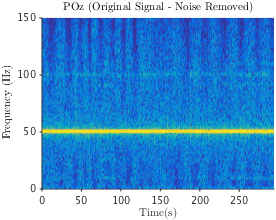
\includegraphics[width=0.4\textwidth]{images/3-3-d-2.pdf}
	\caption{Spectrogram of difference between original and noise removed graph.}
	\label{fig:3-3-d-2}
\end{figure}



%TODO: write this up a little more nicely.

\end{document}
